\section{Performance Introspection}\label{sec:overview}

\ds{Some parts of this section might need to be lifted into the Intro.}
Specialized OS policies can provide performance gains for specific contexts but pose the risk of silent performance degradations under contexts that deviate even slightly.
% The core challenge in enabling performance reliability for specialized OS policies today is the lack of performance signals in the OS.
Today, the only practical way for operators to build confidence in specialized OS policies \aditya{this is imprecise. what does build confidence mean? be clear about what operators are trying to do with specialized policies and what blind spots/issues they face when using them.} is through extensive offline evaluation across many workloads, followed by manual inspection of end-to-end performance metrics.
This process is expensive, incomplete, and ultimately unsatisfactory: no finite offline evaluation can anticipate the diversity of executions encountered in deployment.

We argue that ensuring performance reliability for specialized OS policies requires a different capability altogether: rather than relying solely on offline testing and analysis, the OS should be able to introspect whether its policies are behaving well {\it at run-time}, using signals available during execution, and intervene when they are not. We call this capability {\it \textbf{performance introspection}}.
In this paper, we propose a framework that brings such run-time performance introspection capabilities to the OS.
The key building blocks enabling this framework are {\it \textbf{OS Guardrails}}.

\aditya{i don't like the specialization story.
isn't any policy "specialized" by definition or design?
also, note that beyond 3.0 there is no mention of specialization, so why bring it up in the first place
just say that policies are brittle from a perf perspective because designers are forced to make assumptions about workloads, enviornments etc that easily break at deployment time or in production. thus we need a principled way of knowing when that's happening and taking appropriate actions.}

% In the rest of this section, we first describe the workflow for performance introspection in our framework, explaining the guardrail primitive (\Cref{subsec:framework}), and then provide a formal basis for how run-time guardrails can provide performance reliability (\Cref{subsec:formal-basis}).

% A very successful technique has been to use formal verifiers before being deployed~\cite{certikos-osdi16}, or offline testing approaches can provide coverage over contexts of interest for the given policy\ds{add testing based cites}.
% One straightforward way to enable runtime signals about OS performance would be to have applications communicate explicit information about their achieved performance. However, besides breaking the current application-OS interface, this approach has a major flaw: simply providing end-to-end application performance indicators leaves no way for the OS to figure out which policy to improve. 
% Thus, such signals neither use readily available statistics nor are they actionable.

\subsection{OS Guardrails}\label{subsec:guardrails-desc}

An OS Guardrail (or guardrail, for simplicity) is a construct that evaluates whether the execution of an OS policy meets the requirement of reliable performance.
A guardrail captures two things: (i) a performance property that should hold for a policy or subsystem, and (ii) a corrective action to take when that property is violated.
We provide an intuitive explanation here, and give a detailed formal definition in \Cref{sec:gdl}.

We use the term \emph{performance property} to denote a measurable \eric{safety?}predicate over policy execution in the OS.
Depending on the policy, this predicate may be expressed over the policy’s inputs, its outputs, or the resulting system state.
For instance, a hugepage allocator may target low allocation latencies (captured by execution time statistics); a network flow scheduler with a learned flow size predictor may require high prediction accuracy (captured by the immediate outputs of the predictor); and a memory tiering policy may require high DRAM bandwidth utilization (captured by system statistics that result from using the policy).
These examples demonstrate the same underlying idea: the OS should be able to determine, from run-time evidence, whether the policy is operating in a desirable regime.

Corrective actions similarly depend on the policy and the failure mode being guarded against.
For instance, if a hugepage allocator takes too long, then the action may be to revert to the basepage allocator; if a predictor for flow sizes is resulting in inaccurate outputs, then the action may be to retrain the existing model; and if the memory tiering policy has low DRAM bandwidth utilization, then the action may be to promote pages more aggressively. \aditya{all of these are reactive actions. shouldn't we have proactive ones that deny an action}


\subsection{Principles for Designing Useful Guardrails}\label{subsec:principles}

\ds{A high-level question that I haven't answered head on is: why should guardrails be separate and not a part of the policy itself. Suggestions?}
\eric{Can probably borrow some motivation from Aspect Oriented programming https://en.wikipedia.org/wiki/Aspect-oriented_programming}
\sujay{As discussed, guardrails are more of an enhancement than a safeguard. We should mention this here or elsewhere.}
Guardrails are as useful as the properties they monitor -- thus, designing good properties is key to building useful guardrails.
We propose two principles for designing useful guardrails:
\begin{densenumerate}
\item Properties must be based on performance signals observable at run time within the OS.
\item Properties should capture the absence of undesirable behavior rather than prescribe ideal behavior.
\end{densenumerate}

% There are two guidelines we propose to design good performance properties.
To illustrate these principles and provide justification for them, we use transparent hugepage promotion (THP) as a running example.
For a hugepage promotion policy, the goal is to decide which set of contiguous pages to promote into a hugepage and when. Hugepages help by reducing TLB miss rates and hence, save page walk cycles, but these savings must also be balanced against the overhead of allocating hugepages~\cite{cbmm-atc22}.
A common method of specifying performance targets today is via tail-latency SLOs, as follows: `the 99th percentile execution time for any given workload when running the new policy should be at most 100 milliseconds'.

However, a property on application tail-latency SLOs is difficult for the OS to evaluate: it requires application-visible metrics, that break the application-OS interface.
\sujay{Instead, the guardrail should monitor the hugepage allocator latency to ensure its below a threshold.}
More generally, a property is useful for run-time performance introspection only if the OS can evaluate it during execution.
This restriction leads us to the first principle above.
Note that this principle rules out performance specified using end-to-end objectives that require external measurement, or properties whose validation is inherently offline, such as eventual convergence guarantees or long-horizon notions of fairness.
Such properties are still important, but they cannot serve as the basis for run-time performance introspection.

The second problem with the SLO-based performance property is that the SLO thresholds must vary with the workloads.
Thus, specifying a threshold for `ideal' performance is difficult. \aditya{this example is unclear. it is not obvious what ideal and bad means in this case and why one is difficult vs the other.}
In contrast, it is often much easier to identify clearly undesirable behavior -- operators and OS policy developers can use their domain knowledge to express invariants such as `at least this behavior should not happen'. \aditya{this is an ill-formed phrase}
This illustrates our second principle above. \aditya{inline these explanations with the principles. easier to follow and tighter.} \eric{I think an example would also make this easier to follow}

Taking these guidelines into account, a more useful guardrail can then be designed by specifying poor behavior that should not occur in any THP policy.
For example, if a THP policy repeatedly allocates hugepages that are never accessed, then the cycles spent in allocating them are necessarily wasted (and hence, a signal of poor policy performance).

\begin{figure}
    \centering
    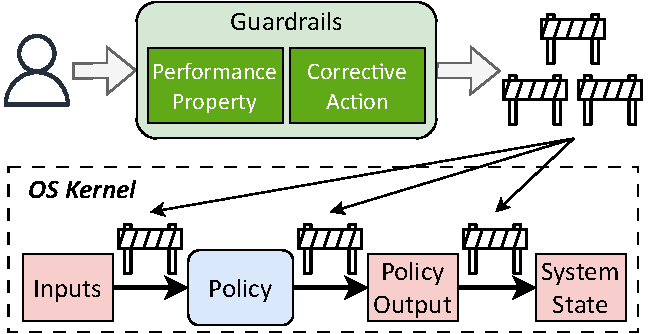
\includegraphics[width=0.9\columnwidth]{figures/Overview/overview.pdf}
    \caption{Overview of Guardrails}
    \label{fig:framework-overview}
\end{figure}

\subsection{Workflow and Key Components}\label{subsec:framework}

The above discussion shows that OS guardrails should be expressed as precise, executable specifications over OS-visible behavior.
This, in turn, imposes certain requirements needed to support performance introspection in the OS: guardrails must be specified declaratively, compiled into efficient monitors, and integrated directly into the execution path of OS policies.
We propose a framework that achieves these requirements. We explain this using the workflow depicted in~\Cref{fig:framework-overview}.

\aditya{the rest of this is good, but a bit verbose}
For each specialized policy (or subsystem) of interest, our framework requires operators to specify the guardrails, consisting of desired performance properties and corresponding corrective actions.
Today, there exists no mechanism for operators to specify the performance properties they require of the OS or the actions to take when the performance is poor.
The central challenge is therefore to provide an intuitive yet expressive interface for operators, while remaining implementable using run-time statistics.
Our framework addresses this challenge via the {\it \textbf{Guardrail Description Language (\lang)}}, a domain-specific language designed around typical OS abstractions such as kernel objects, kernel functions, and run-time statistics.
To ensure that properties can be evaluated at run time with low overhead, \lang uses primitives that restrict performance properties to predicates over kernel-visible features that are observable during execution (e.g., per-object counters, latency measurements, and scheduling or memory-state signals).

At run time, \lang guardrails are compiled into {\it \textbf{Guardrail Monitors}} that operate alongside the policy execution path, as depicted in Figure~\ref{fig:framework-overview}.
As inputs drive policy decisions and update system state, these monitors continuously evaluate the specified predicates over the resulting execution trace.
In order to make the varied statistics, necessary for evaluating properties, readily available, we maintain an in-kernel feature store, as proposed previously in LAKE~\cite{lake-asplos23}.
We implement these monitors using \texttt{eBPF}, enabling efficient in-kernel execution, low deployment overhead, and dynamic updates to guardrail logic.
When a predicate evaluates to false, the guardrail is said to be triggered, and this results in the execution of its prescribed corrective action, steering the policy back toward its intended operating regime.